\documentclass[11pt,a4paper]{article}
\usepackage[top=2.5cm, bottom=2.5cm, left=2.5cm, right=2.5cm]{geometry}
\usepackage{tikz}
\usetikzlibrary{arrows.meta}
\usepackage[numbers,sort&compress]{natbib}
\usepackage{array}
\usepackage{booktabs}
\usepackage{caption}
\usepackage{hyperref}

\begin{document}

\title{Timeline of the Matrix Multiplication Exponent $\omega$}
\author{}
\date{}
\maketitle

The exponent $\omega$ is defined so that two $n \times n$ matrices can be multiplied
in $O(n^{\omega})$ field operations. The trivial bounds are $2 \le \omega \le 3$;
the lower bound comes from the $2n^2$ entries that must be read, and the upper
bound from the schoolbook algorithm.

\begin{figure}[h]
\centering
\resizebox{\textwidth}{!}{%
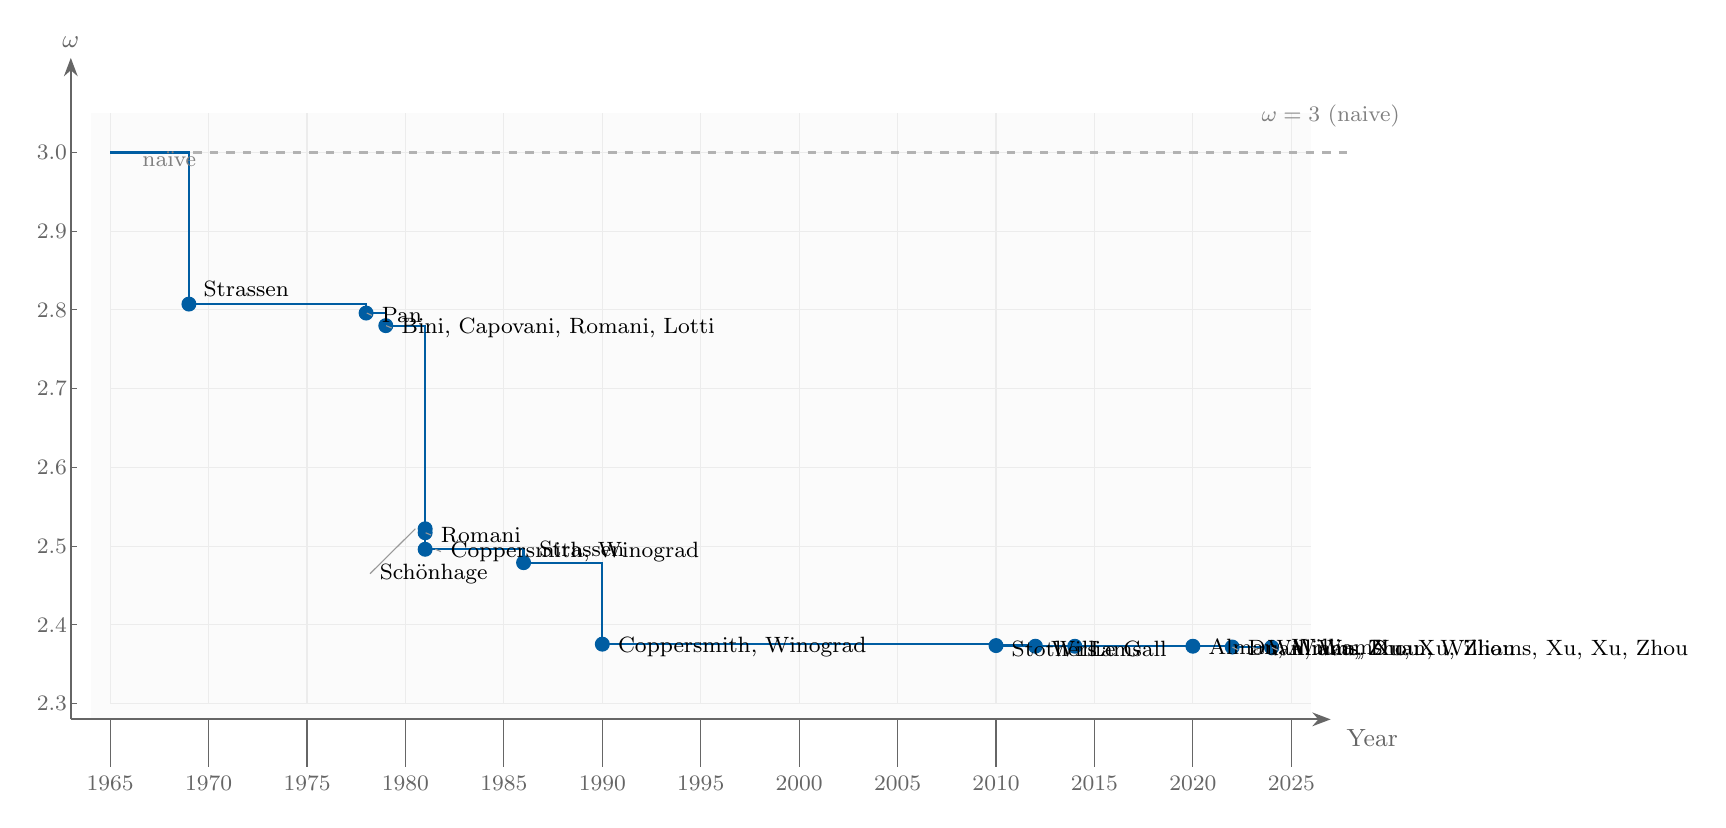
\begin{tikzpicture}[
  x=0.25cm, y=10cm,
  font=\small,
  >=Stealth,
]
% Coordinate system: X = year - 1960, Y = omega - 2

% --- Plot area background ---
\fill[gray!3] (4, 0.28) rectangle (66, 1.05);

% --- Axes ---
\draw[->, thick, black!60] (3, 0.28) -- (67, 0.28) node[below right, xshift=2pt] {Year};
\draw[->, thick, black!60] (3, 0.28) -- (3, 1.12)  node[above] {$\omega$};

% --- Grid ---
\foreach \x in {5,10,15,20,25,30,35,40,45,50,55,60,65}
  \draw[gray!15] (\x, 0.3) -- (\x, 1.05);
\foreach \y in {0.3,0.4,0.5,0.6,0.7,0.8,0.9,1.0}
  \draw[gray!15] (5, \y) -- (66, \y);

% --- Reference line ---
\draw[dashed, thick, black!30] (5, 1) -- (68, 1);

% --- Tick labels ---
\foreach \x/\yr in {5/1965,10/1970,15/1975,20/1980,25/1985,30/1990,
                     35/1995,40/2000,45/2005,50/2010,55/2015,60/2020,65/2025}
  \draw[black!60] (\x, 0.28) -- (\x, 0.22) node[below, font=\footnotesize] {\yr};
\foreach \y/\w in {0.3/2.3,0.4/2.4,0.5/2.5,0.6/2.6,0.7/2.7,0.8/2.8,0.9/2.9,1.0/3.0}
  \draw[black!60] (3, \y) -- (3.3, \y) node[left, font=\footnotesize] {\w};

% --- ω=3 label ---
\node[above, font=\footnotesize, black!50] at (67, 1.02) {$\omega = 3$ (naive)};

% --- Step path ---
\draw[thick, color={rgb:red,0;green,0.4;blue,0.7}] (5,1)
  -- (9,1) -- (9,0.8074)
  -- (18,0.8074) -- (18,0.796)
  -- (19,0.796) -- (19,0.780)
  -- (21,0.780) -- (21,0.522)
  -- (21,0.517) -- (21,0.496)
  -- (26,0.496) -- (26,0.479)
  -- (30,0.479) -- (30,0.3755)
  -- (50,0.3755) -- (50,0.3737)
  -- (52,0.3737) -- (52,0.3729)
  -- (54,0.3729) -- (54,0.3728639)
  -- (60,0.3728639) -- (60,0.3728596)
  -- (62,0.3728596) -- (62,0.371866)
  -- (64,0.371866) -- (64,0.371552)
  -- (64,0.371339);

% --- Data points ---
\foreach \point in {
  (9,0.8074), (18,0.796), (19,0.780),
  (21,0.522), (21,0.517), (21,0.496),
  (26,0.479), (30,0.3755),
  (50,0.3737), (52,0.3729), (54,0.3728639),
  (60,0.3728596), (62,0.371866),
  (64,0.371552), (64,0.371339)}
  \filldraw[fill={rgb:red,0;green,0.4;blue,0.7},
            draw={rgb:red,0;green,0.4;blue,0.7}] \point circle (2.5pt);

% --- Labels with leader lines (matching Wikipedia style) ---

%% Naive label (at ω=3, year 1965--1969)
\node[above, font=\footnotesize, black!50] at (8,0.97) {na\"ive};

%% Strassen 1969
\node[above right, font=\footnotesize] at (9.25,0.804) {Strassen};

%% Pan 1978
\draw[thin, black!40] (18.033,0.796) -- (18.3,0.793);
\node[right, font=\footnotesize] at (18.3,0.793) {Pan};

%% Bini--Capovani--Romani 1979
\draw[thin, black!40] (19.016,0.780) -- (19.3,0.777);
\node[right, font=\footnotesize] at (19.3,0.777) {Bini, Capovani, Romani, Lotti};

%% 1981: Sch\"onhage (placed in the gap before the drop)
\draw[thin, black!40] (20.5,0.522) -- (18.2,0.465);
\node[right, font=\footnotesize] at (18.2,0.465) {Sch\"onhage};

%% Romani
\draw[thin, black!40] (21.025,0.517) -- (21.3,0.514);
\node[right, font=\footnotesize] at (21.3,0.514) {Romani};

%% Coppersmith, Winograd (1981)
\draw[thin, black!40] (21.516,0.496) -- (21.8,0.493);
\node[right, font=\footnotesize] at (21.8,0.493) {Coppersmith, Winograd};

%% Strassen 1986
\node[above right, font=\footnotesize] at (26.3,0.475) {Strassen};

%% Coppersmith, Winograd 1990
\node[right, font=\footnotesize] at (30.3,0.372) {Coppersmith, Winograd};

%% Post-2010
\node[right, font=\footnotesize] at (50.3,0.370) {Stothers};
\node[right, font=\footnotesize] at (52.3,0.370) {Williams};
\node[right, font=\footnotesize] at (54.3,0.370) {Le Gall};
\node[right, font=\footnotesize] at (60.3,0.370) {Alman, Williams};
\draw[thin, black!40] (62.008,0.3719) -- (62.3,0.368);
\node[right, font=\footnotesize] at (62.3,0.368) {Duan, Wu, Zhou};
\draw[thin, black!40] (63.033,0.3716) -- (63.3,0.368);
\node[right, font=\footnotesize] at (63.3,0.368) {Williams, Xu, Xu, Zhou};
\draw[thin, black!40] (64.016,0.3713) -- (64.3,0.368);
\node[right, font=\footnotesize] at (64.3,0.368) {Alman, Duan, Williams, Xu, Xu, Zhou};

\end{tikzpicture}%
}
\caption{Improvement of the best known upper bound on the matrix multiplication
exponent $\omega$ over time. The dashed reference line shows the trivial upper
bound $\omega \le 3$ of the schoolbook algorithm.}
\label{fig:omega}
\end{figure}

\begin{table}[h]
\centering
\caption{Timeline of advances in the matrix multiplication exponent $\omega$.}
\label{tab:omega}
\small
\begin{tabular}{c>{\raggedright\arraybackslash}p{3.6cm}>{\raggedright\arraybackslash}p{3.6cm}c}
\toprule
Year & $\omega$ upper bound & Authors & Ref. \\
\midrule
1969 & 2.8074    & Strassen                              & \cite{strassen1969}            \\
1978 & 2.796     & Pan                                   & \cite{pan1978}                 \\
1979 & 2.780     & Bini, Capovani, Romani, Lotti          & \cite{bini1979}                \\
1981 & 2.522     & Sch\"onhage                           & \cite{schonhage1981}           \\
1981 & 2.517     & Romani                                & \cite{romani1981}              \\
1981 & 2.496     & Coppersmith, Winograd                 & \cite{coppersmith1982}         \\
1986 & 2.479     & Strassen                              & \cite{strassen1986}            \\
1990 & 2.3755    & Coppersmith, Winograd                 & \cite{coppersmith1990}         \\
2010 & 2.3737    & Stothers                              & \cite{stothers2010}            \\
2012 & 2.3729    & Williams                              & \cite{williams2012}            \\
2014 & 2.3728639 & Le Gall                               & \cite{legall2014}              \\
2020 & 2.3728596 & Alman, Williams                       & \cite{alman2020}               \\
2022 & 2.371866  & Duan, Wu, Zhou                        & \cite{duan2022}                \\
2024 & 2.371552  & Williams, Xu, Xu, Zhou                & \cite{vxxz2024}                \\
2024 & 2.371339  & Alman, Duan, Williams, Xu, Xu, Zhou   & \cite{alman2024}               \\
\bottomrule
\end{tabular}
\end{table}

\bibliographystyle{abbrv}
\bibliography{refs}

\end{document}
